\documentclass[letterpaper,conference]{IEEEtran}

\usepackage[margin=1.14in]{geometry}
\usepackage{graphicx,url}
\usepackage{amsthm}
\usepackage{listings}
\newtheorem{definition}{Definition}


\hyphenation{op-tical net-works semi-conduc-tor}

\begin{document}

\title{Quality-Aware Context Provider: A filtering approach to context-aware systems on ubiquitous environment}
\author{\IEEEauthorblockN{Caio Silva and M.A.R Dantas}
\IEEEauthorblockA{Research Laboratory of Distributed Systems (LaPeSD)\\ 
Department of Informatics and Statistic (INE)\\
Federal University of Santa Catarina (UFSC)\\
88040-900 – Florianópolis, SC – Brazil\\
caio.cmsilva@gmail.com, mario.dantas@ufsc.br}
}

\maketitle

\begin{abstract}
In ubiquitous environment context awareness approach plays a vital role in adaptability
to user’s requirements. Context-sensitive systems meet specific requirements correctly, 
only if context information possesses the desired quality of context (QoC). Context data
can be unreliable or inaccurate, thus undermining the potential of context-aware 
services. Some researches adopt a conflict resolution approach through the utilization 
of few QoC parameters. Other studies define policies based on QoC parameters to resolve 
conflicts. Both efforts do not exploit application requirements to ensure quality of 
context. In this research work it is proposed a QoC filtering approach. Our proposal 
intends to use in a better fashion the context provider, sending only relevant data to 
the context server. Besides that we present QoC policies, based in terms of application 
requirements and QoC parameters, which are used in a validation process to filter 
context data. The experimental simulation indicates a reduction in the amount of data 
sent and also an improvement on the quality of context on transmitted data.
\end{abstract}

\begin{IEEEkeywords}
context-aware systems, quality of context, ubiquitous computing
\end{IEEEkeywords}

\IEEEpeerreviewmaketitle

\section{Introduction}

 Ubiquitous computing is a paradigm characterized by the presence of portable devices, 
 which are increasingly part of the day-to-day lives. These devices have considerable 
 processing power, storage space and wireless communication capabilities. In addition 
 to that, this equipment has diverse functionalities and interfaces as GPS, Bluetooth, 
 accelerometer, audio players, and digital cameras. These features have a strong link 
 with the physical world, and the information provided by them can be used to provide 
 services with fully awareness of current execution environment. The information 
 captured from user environment is usually called context and represent the input 
 element for context-sensitive computing \cite{nazario2012taxonomia}.

Context-awareness permits mobile services to dynamically and efficiently adapt both to 
the current situation, such as current physical place and/or social activity, and to 
the challenging and highly variable deployment conditions typical of mobile environments
(e.g. resources scarcity, unreliable and intermittent wireless connectivity) \cite{bellavista2013survey}. 
A context-awareness approach can, also, minimize power consumption, processing time and 
the amount of data propagated over the network, optimizing the use of computational resources.

However, context information has an innate characteristic of imperfection and its 
quality is highly influenced by the way it is gathered. In fact, it may even be 
incorrect. Most sensors feature an inherent inaccuracy (e.g., a few meters for GPS 
positions), and the sensed values age if the physical world changes, so that this 
inaccuracy increases over time. For instance, raw sensed data can be affected by many 
error sources, such as unavailability, inapplicability, external influences (e.g., 
temperature, interferences), and context refinement operations (e.g., fusion, reasoning)
\cite{henricksen2004modelling}.

Imperfect and conflicting context data may hinder the proper functioning of 
context-sensitive applications. Quality of context (QoC) principles can be used to 
tackle conflicting situations. Some researches, as shown in \cite{buchholz2003quality} \cite{sheikh2007middleware} \cite{klein2010time} \cite{neisse2008trustworthiness} 
\cite{manzoor2008evaluation} \cite{tang2007context}, propose solutions for collecting, 
representing, and evaluating QoC indicators. However, little attention has been given 
to the use of QoC to resolve context conflicts. 

Manzoor et al. \cite{manzoor2009using} present conflict resolving policies that are 
defined on the basis of the quality of context parameters. We consider that conflict 
resolving policies should be used to improve quality on context information. Therefore, 
policies must be designed on the basis of context model parameters. Filho et al. \cite{agoulmine2011quality} 
propose an approach to resolve internal and external context conflicts based on two QoC 
indicators: probability of correctness and trustworthiness. We believe that a conflict 
resolution approach should use all available QoC indicators to ensure the desired quality.

Nevertheless, even with these approaches, the context provider still sends a large 
amount of context data that is redundant, conflicting, and unreliable or does not have 
the information desired by a context consumer. Such information are not required to be 
sent through the network to context consumers, the pervasive device itself can take 
some responsibility on validating the data produced.

As a result, this proposal seeks to use in a better fashion the context provider (CP), 
sending only useful information to the context server, ensuring a better quality of 
context and optimizing the use of device features. We consider that the detection and 
resolution of conflicts should also be performed by the context provider in order to 
reduce the probability of propagating errors to the upper context management layers.

In this paper a differentiated approach is presented. The research proposal considers 
the filtering process of context data before sending them to a context server. The 
context provider has the responsibility to remove redundant and conflicting data. CP 
uses quality of context policies to perform a validation process on recently captured 
data, thus discarding useless information. Consequently, less data are sent through the 
network, increasing substantially server scalability and significantly decreasing 
computational efforts to process and identify conflicting data. 

The remainder of this paper is organized as follows. Section II presents a brief
discussion about context middleware. The proposed model and QoC policies definitions are 
described in section III. In section IV it is presented a set of experimental results. 
Finally, conclusions and discussions of future work are shown in section V.

 \section{Context-Aware Middlewares} 

% This section presents the basic concepts involving context-awareness and quality of 
% context. Furthermore, we conduct a brief discussion about how a context middleware 
% interacts with hardware infrastructure and applications, as well as how context data 
% propagate through system layers.

% \subsection{Context and QoC Concepts}
% 
%  Context is still a vague concept to identify the aspects the designer considers useful 
%  to model and describe the environment where a given service is to be deployed and 
%  executed \cite{bellavista2013survey}. 
% There are several classifications of context in the literature such as those found in  
% \cite{dey2000providing} \cite{schilit1994context} \cite{zimmermann2007operational} 
% and \cite{bolchini2009context}. We adopted the context definiton presented in \cite{chen2000survey},
% where context is a four-dimensional space composed by: 
% 
% \begin{itemize}
%  \item \textit{Computing context}: Deals with all those technical aspects related to computing
%        capabilities and resources;
%  \item \textit{Physical context}: Groups all those aspects that represent real world and that are
%        accessible by using sensors/resources deployed in the node surroundings;
%  \item \textit{Time context}: Captures the time dimension, such as time of a day, week, month, and
%        season of the year, of any activity performed in the system (either real-world or
%        computing);
%  \item \textit{User context}: contains high-level context aspects related to the social
%        dimension of users, such as user’s profile, people nearby, and current social 
%        situation;
% \end{itemize}
% 
% Thus, considering all the context dimensions mentioned, different context behaviors can 
% be accomplished to adapt services to make them suitable for the end user and to conform 
% current execution environment characteristics. For this purpose, quality of context data
% is a key issue, since it may impair the correctness of adaptations operations \cite{bellavista2013survey}. 

% Quality of Context (QoC) is any information that describes the quality of the 
% information being used as context information. Thus, QoC refers to information and 
% neither to the process nor the hardware component that possibly provide the information.
% Consequently, the emerging notion of Quality of Context (QoC) usually defined as the set
% of parameters that express quality requirements and properties for context data (e.g.,
% precision, freshness, trustworthiness) is overwhelming important to control and manage 
% all the possible context inaccuracies \cite{buchholz2003quality} \cite{krause2005challenges}.
 
% Several researches are being conducted to identify and evaluate relevant information to ensure quality 
% of context \cite{klein2010time} \cite{manzoor2008evaluation} \cite{neisse2008trustworthiness}  \cite{brgulja2009measuring}
% \cite{kim2006quality} \cite{miron2010modeling}. Usually, in the literature, quality of 
% context information is presented as QoC parameters. Each application has its own scope 
% of quality parameters. However, some parameters presented in the literature are useful 
% for a wide range of applications. Some of them are: i) up-to-dateness to deal with data
% aging; ii) trustworthiness to rate the belief we have in context correctness; iii) 
% completeness to consider that context data could be partial and so incorrect; and iv) 
% significance to express differentiated priorities \cite{bellavista2013survey}.

% As it is described in \cite{buchholz2003quality}, quality of context (QoC) is any information 
% that describes the quality of the information being used as context information. Consequently,
% quality of context refers to the quality of context data and also to the quality of data 
% distribution. Without an efficient data distribution, it is not feasible the deployment of 
% truly context-aware services. Thus, the context provider must have some guarantees on context 
% data distribution, anticipating the occurrence of some adverse situations (e.g., 
% disconnection, lack of signal, roaming).

% Context information and quality parameters are related through a quality of context 
% (QoC) model. A QoC model establishes: which is the information that must be taken 
% into account to describe the environment where information is captured. Furthermore, 
% a quality model should present all the relations between context attributes and QoC 
% parameters. This winning combination of attributes and relationships describe the set 
% of context information demanded by a context-aware service/application.
 
% Hence, similarly to context-awareness in itself, a well-accepted QoC definition is 
% still missing. Several authors presented their own QoC framework, also introducing 
% and using the same concepts with different names. However, despite these differences, 
% a common thought can be highlighted: QoC is not requiring perfect context data, such 
% as all data with the highest possible precision and up-to-dateness, but having and 
% maintaining a correct estimation of the data quality \cite{buchholz2003quality}.

% \subsection{Context-Aware Middleware}

 In this section, we raise some concepts related to context middleware, in order to 
 characterize the scenario which fits our proposal. 
 
 In \cite{kjaer2007survey} it is defined as a general middleware as software system which 
 provide an abstraction layer between an operating system and applications running in a 
 distributed environment. More specifically, a context middleware aim to manage, in a 
 transparent way, all major phases of management involved in the provision of context data
 for context-sensitive consumers, i.e., representation, aggregation, distribution, 
 quality assurance, etc.  \cite{baldauf2007survey}.
% 
%  \begin{figure}[!ht]
%  \centering
%   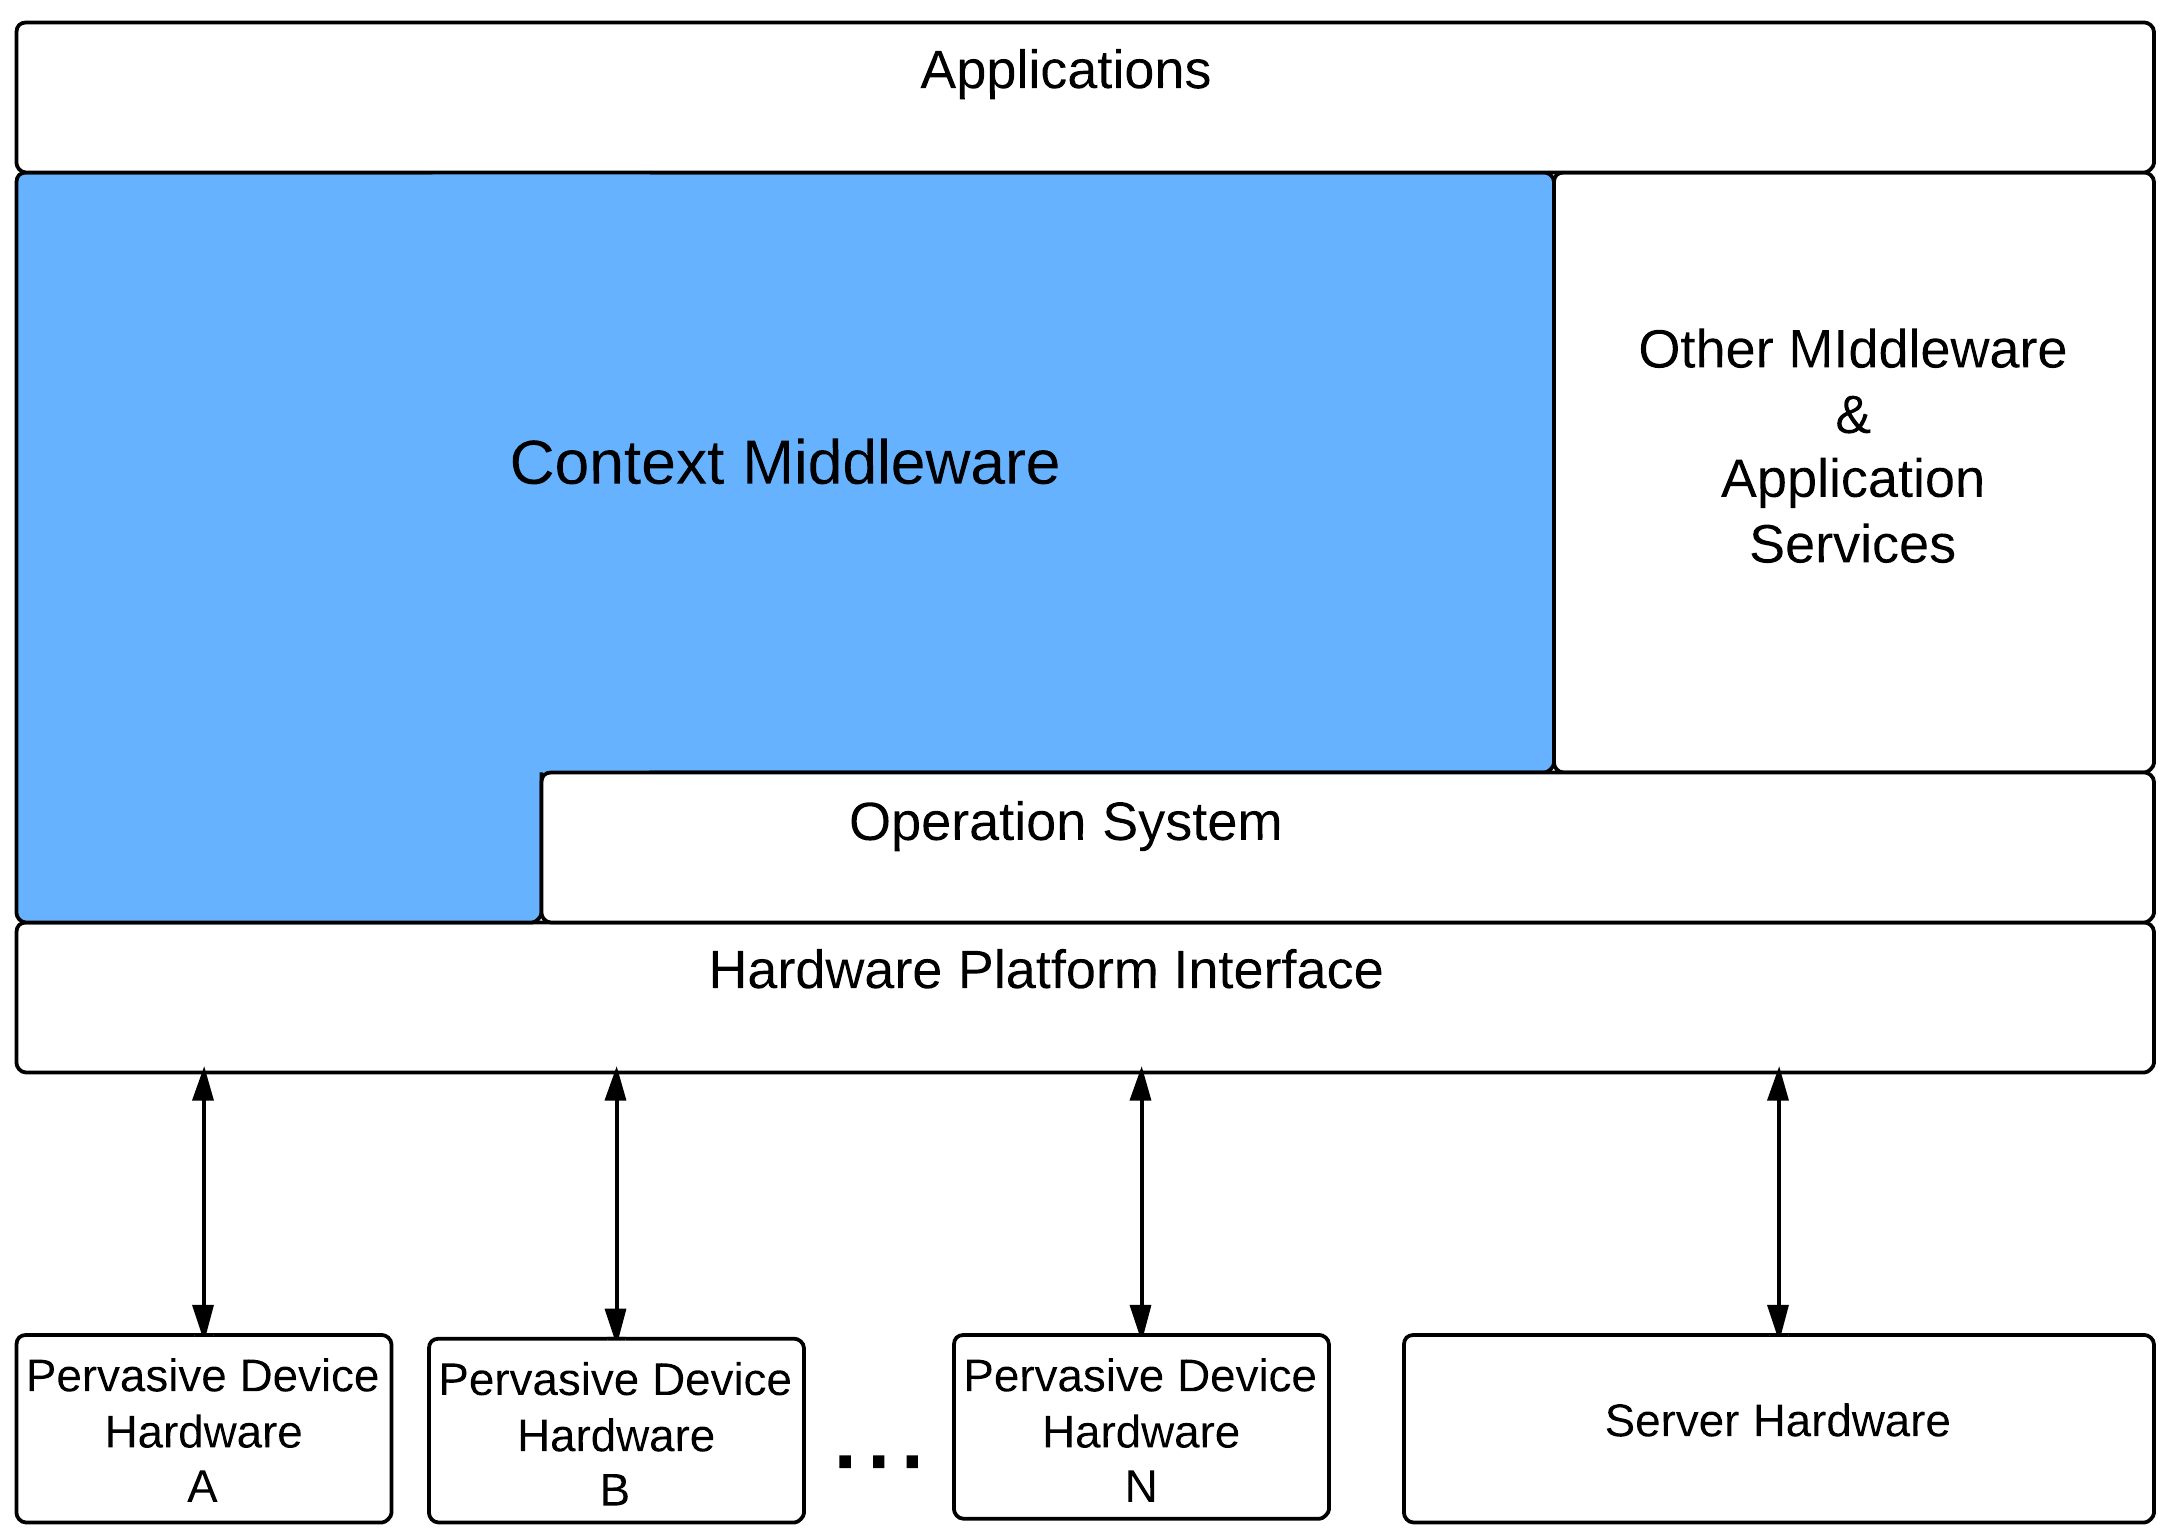
\includegraphics[scale=0.1]{imagens/ContextArq}
%  \caption{Context-Aware System Logical Architecture}
%   \label{contextarq}
%  \end{figure}
% 

 Pervasive devices are usually used as raw context information providers. However, 
 considering the computational power found on nowadays pervasive devices, we suggest 
 that the context-aware middleware should also explore the hardware infrastructure of 
 these devices. The computational capabilities of pervasive devices can be used to improve 
 QoC in context-aware applications. In a more comprehensive, exploiting pervasive device 
 facilities into context middleware improves the quality of provided service in means of:
% 
 \begin{itemize} 
  \item \textit{Interoperability:}  Data provided by pervasive devices in heterogeneous 
 				    environments are created and communicated based on 
 				    the specific pattern of each device. The devices can 
 				    be explored to provide standardized and interoperable
 				    context information across the context middleware.
  
  \item \textit{Distribution:}      Wireless communication is susceptible to issues such 
 				    as temporary disconnection, frequent topology changes,
 				    and limited delivery guarantees. Coordination and 
 				    dissemination protocols should be implemented on 
 				    pervasive devices, as well as methods and algorithms 
 				    to properly deliver the context data.
 				    
  \item \textit{Quality of Context:} Context providers typically provide context 
 				     information within a defined scope. Specific 
 				     algorithms and policies based on quality parameters 
 				     can be used to qualify the data provided by these 
 				     devices, taking into account all device limitations.
 				     
  \item \textit{Storage:}          Mobile devices have considerable storage capability. 
 				   The adaptation process may occur more quickly if 
 				   devices stores context data, since the access is 
 				   locally made. Furthermore, in case of limited connection, 
 				   device storage can also be used to store context data until 
 				   the data can be forwarded. 
 \end{itemize}
 
 
  Therefore, a context-aware middleware should provide quality context data for the 
  applications it supports. We believe that ensuring quality of 
  context is not limited to evaluation of quality parameters and guarantees on data 
  distribution. Application needs must also be taken into consideration to ensure 
  effectively qualified data.
  
 Even with the quality of context ensured, context information may not be desired by 
 the application such information can be conflicting and redundant. A conflict occurs
 when two (or more) context data provide different information about a certain situation.
 A redundant data is identified by owning the same semantic load of previously submitted
 data.
%  
% %  \begin{figure}[!ht]
% %  \centering
% %   \includegraphics[scale=0.1545]{imagens/ContextDataFlow}
% %  \caption{Context Data Flow}
% %  \label{contextflow}
% %  \end{figure}
%  
%  We use an example to elucidate the concepts of conflicting and redundant context data
%  in application perspective. So, imagine an application that intends to use context information
%  to determine patterns on users’ trajectories.
%   
%    A certain user supplies the application with information using his car GPS and mobile 
%    phone. At time $t_1$, the car GPS informs that the user is at geographic position 
%    $(l_1,l_2)$, and mobile phone, at same time $t_1$, informs that the user is at 
%    $(k_1,k_2)$, where $k_1 \neq l_1$ and $k_2 \neq l_2$, this situation 
%    characterizes a conclict, and must be resolved.
%   
%   Using the same application as example, picture the user at work during $h$ hours. The 
%   mobile device provides information with same semantic value during $h$, in other words, 
%   communicates a set of redundant data, consuming unnecessary computational resources. 
 
  We then consider that the quality of context can only be fully achieved if context 
  models consider application requirements qualifying and distributing only data that 
  contribute to the proper functioning of context-aware services.

\section{Proposal}

 In this section it is presented our quality of context approach. The proposal 
 presentation is divided into three subsections. First, we define QoC policies, 
 and its subcategories. Next subsection, explains the validation process used by 
 the context provider, using simple examples to illustrate some situations where 
 filtering approach can be performed. Finally, the Quality-Aware Context Provider 
 architecture is presented, as well as the functionality of its components.

\subsection{QoC policy definitions}

 Under the assumption that each application has specific goals and given the range 
 of scenarios where context-sensitive applications can be implemented, we believe that 
 it is not possible to guarantee quality of context by applying policies based on only 
 a few quality parameters. For this reason, we define a set of QoC policies that can be 
 used in diverse context-aware scenarios.
 
 \subsubsection{Application Driven Policy}
  
  Application driven policies (AP) are used to define relevant information to  
  context-aware applications. A set of application policies is used to restrict 
  the sample space of a context parameter.
  
  \begin{definition}
   A application policy $AP$ is a tuple $AP = \{c,o,l\}$, where $c$ is a context 
   parameter defined on the context model, $o$ is a comparison operator and $l$ is 
   the limiting value of $c$.
  \end{definition}
  
  For example, an application that uses information provided by a mobile device 
  accelerometer in order to detect movement based on the frequency of human movement 
  (approximately 0 - 10 Hz) \cite{lester2004you}. There is no need to send information 
  when there is no human movement, so application policies $AP = \{frequency, <=, 10 \}$
  and $AP = \{frequency, >=, 0\}$ can be used to reduce the amount of data sent by the 
  mobile device.   
  
 \subsubsection{Quality Parameter Policy}
     
  Quality parameters policies use QoC parameters to assure the quality on context data. 
  Those policies can be static or dynamic, depending on how the parameter is evaluated.
  
  \begin{definition}
    A static QoC policy $SQP$ is a tuple $SQP = \{c, q, o, l\}$ where $c$ is a context 
    parameter defined on the context model, $q$ is a quality of context parameter 
    defined on QoC model, $l$ is the limiting value of $q$ and $o$ is the comparison 
    operator.
  \end{definition}  
  
 Static policies should be used when the value of a QoC parameter can be predefined. 
 Using the accelerometer example, the mobile device should sent information only if the 
 significance \cite{manzoor2008evaluation} of a specific parameter is greater than 85\%, so a QoC policy can be defined as 
 $SPQ = \{frequency,significance,>,0.85\}$.
  
  \begin{definition}
   A dynamic QoC policy $DQP$ is a tuple $DQP = \{c,q,r,o\}$ where $c$ is a context 
   parameter defined on the context model, $q$ is a quality of context parameter 
   defined on QoC model, $r$ is the relation defined to evaluate the QoC paramter 
   and $o$ is the comparison operator.
  \end{definition}

  Dynamic policies should be used in situations where the quality parameter is evaluated
  at runtime. These policies require a high computational power, so it should be used 
  with caution in pervasive devices. We recommend using these policies in context 
  information layer.
  
  Generally speaking, a policy set should be defined for each parameter present on the 
  context model in order to guarantee quality of context on data. In this way, a 
  context parameter can be evaluated by various QoC parameters and report only what 
  applications require.
  

\subsection{Context Validation Process}
 
 In this section it is presented all stages of validation process along with examples, 
 to clarify its comprisement. Figure \ref{validcontext} presents context validation 
 process schema.
 
  \begin{figure}[!ht]
  \centering
  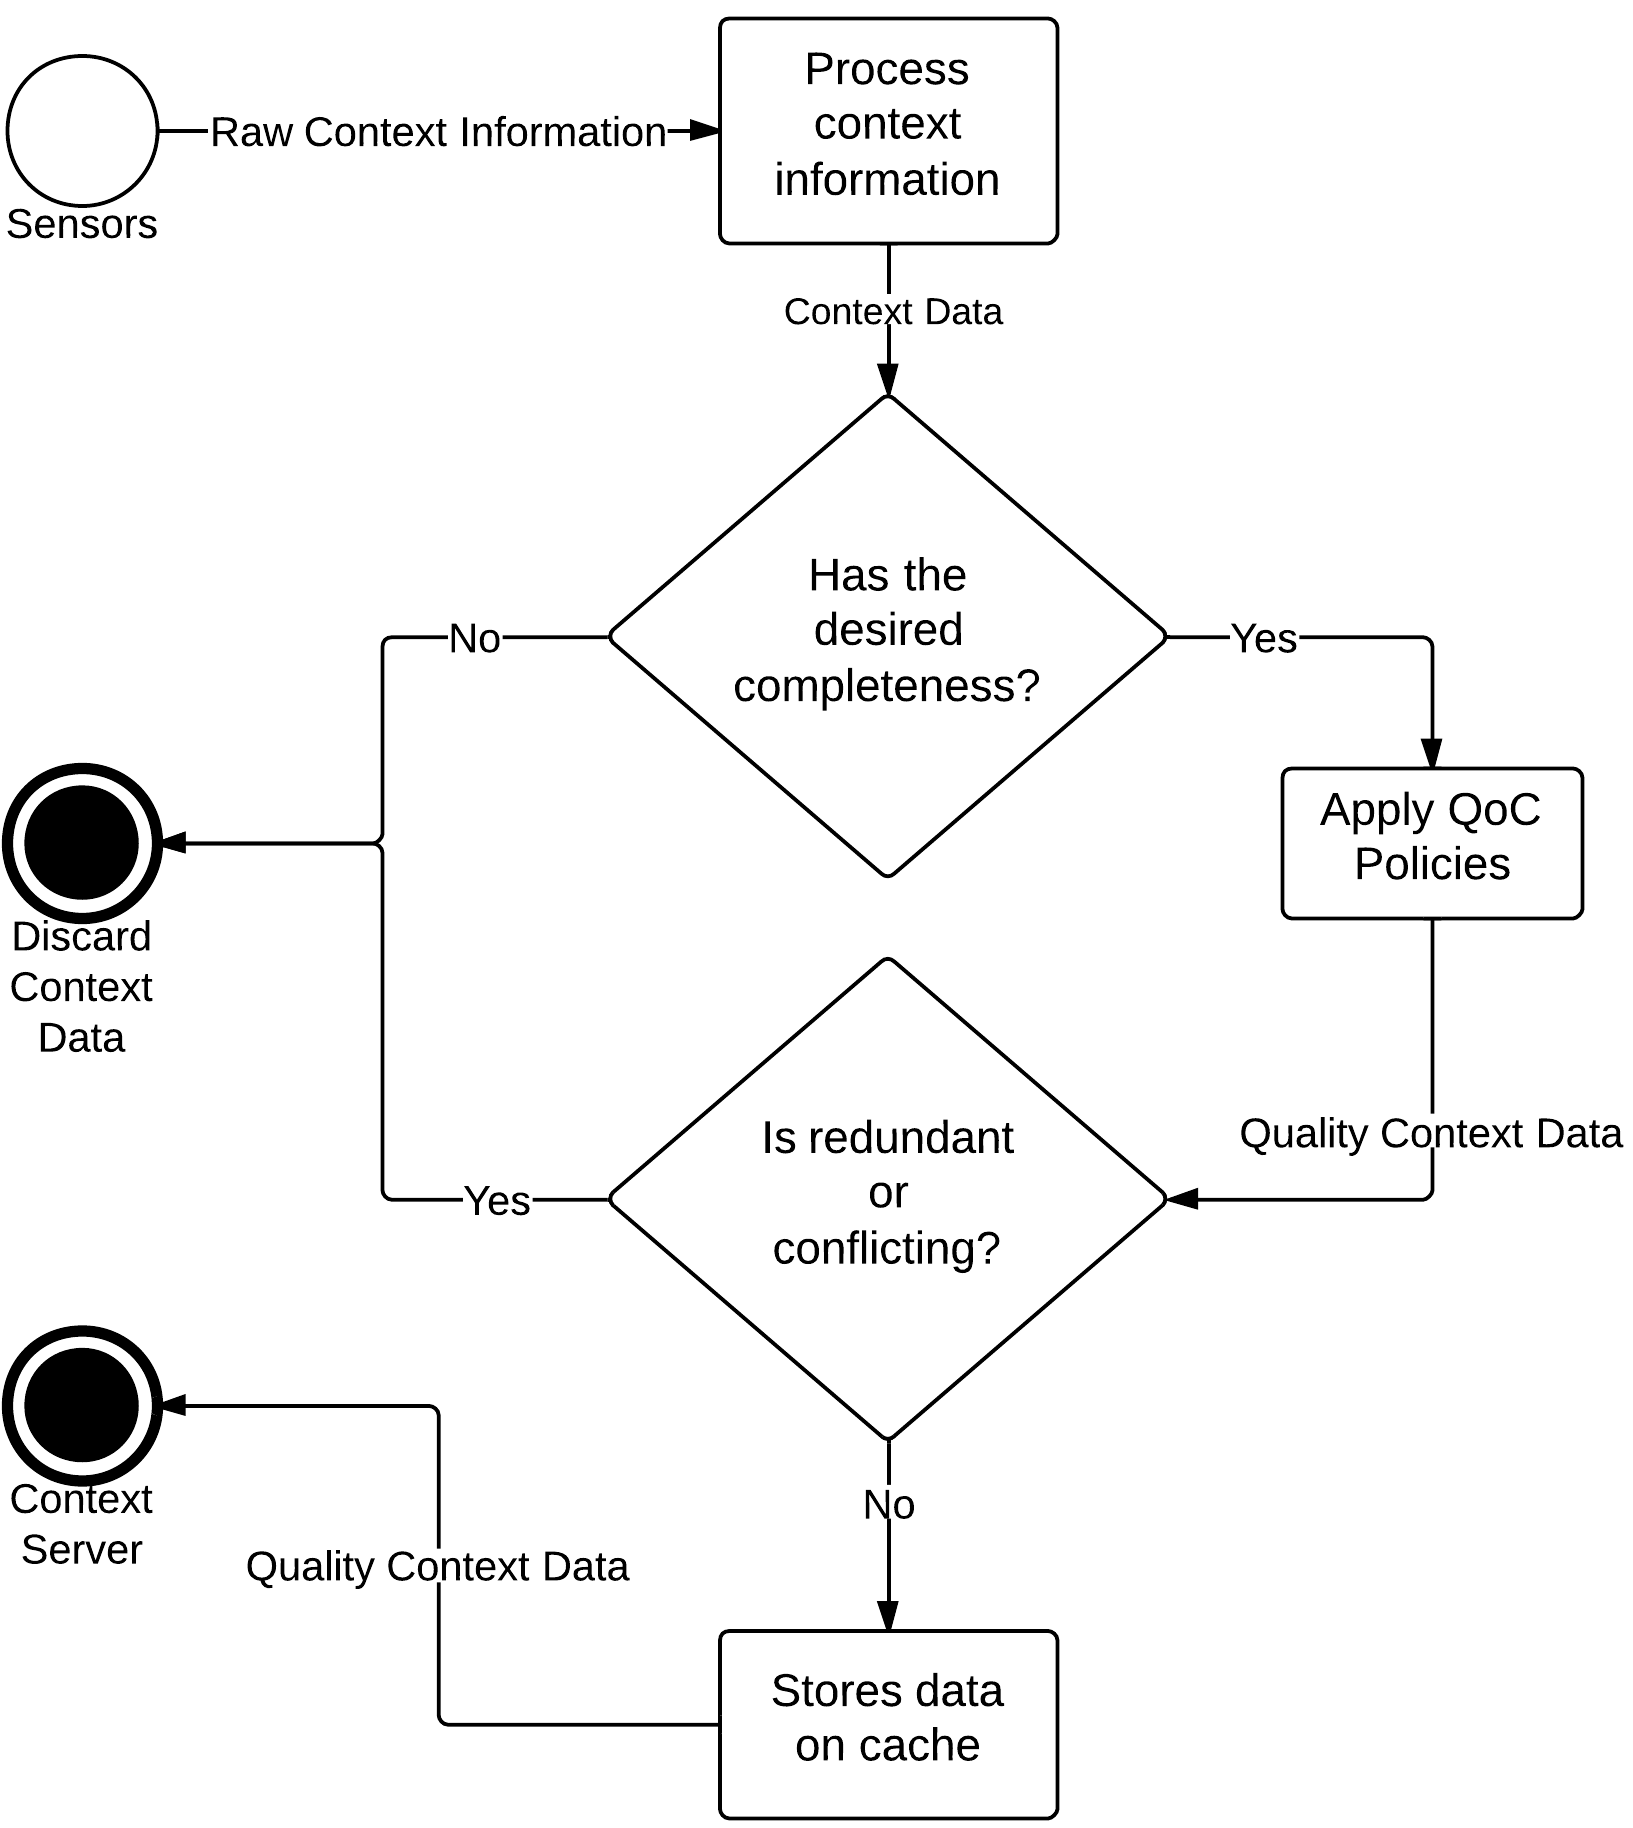
\includegraphics[scale=0.13]{imagens/ContextValidationProcess}
  \caption{Context Data Validation}
  \label{validcontext}
 \end{figure}

 The validation process on context information begins when the context provider receives 
 raw context information from sensors. The information is used to create a context data 
 without any warranty of quality, but still, the newly created data is already 
 interoperable across all context middleware layers.

 Thereafter, the context data is evaluated in terms of completeness, ensuring that all 
 necessary information is available. For example an application that demands information
 about the temperature at a certain time in a certain place. The context data, provided
 via mobile device, must contain all information required by the application, i.e., 
 temperature, time of day and geographic location. Otherwise, the context data is 
 deleted. With all necessary information available, QoC policies are used to ensure 
 quality of context on the context data. Suppose, now, that the aforementioned 
 application is a warning system that alerts users when the temperature exceeds $c$ 
 degrees Celsius in a data center room. Some policies that could be used to achieve 
 the goals of such application and improve the quality of data transferred, would be:
 
 \begin{itemize}
  \item $\{temperature, precision, <=, 1\}$: The temperature precision must be at most 
					      1 degree Celsius.
  \item $\{temperature, significance, >, 0.9\}$: The significance of the temperature 
						  information must be greater than 90\%.
						  For example, if the temperature capture 
						  in $t_n$ is $>>$ than temperature 
						  capture in $(t_\mathit{n-1}, t_\mathit{n-2}, \dots)$ 
						  and $(t_\mathit{n+1},t_\mathit{n+2}, \dots)$, 
						  this information has low significance 
						  and must be discarted. 
  \item $\{temperature, >, 18\}$:  The application does not need data that informs 
				    temperatures below 18 degrees Celsius.
                     
 \end{itemize} 
 
 After the evaluation of quality policies, the quality context data is confronted with 
 recently sent data in order to identify redundancies and conflicts. Returning to the 
 example and assuming that the data center room has stable temperature for a certain 
 period $p$ of day. During $p$, all data created have very similar temperature 
 information, and there is no need to send this redundant information. 
 
 On the other hand, if the temperature exceeds a certain threshold, the application 
 should send information until the situation is resolved. In this case, redundant data 
 are desirables, since a critical condition must be identified by the application. We 
 believe that the characterization of a redundant situation should be done through QoC 
 policies.
 
  As previously mentioned, the information provided by sensors may differ from reality, 
  taking into account the intrinsic inaccuracy found in many of these devices. Such 
 information may cause conflict events. Using the same example as before, imagine that 
 the data center room temperature is stable at $c$ degrees Celsius at a certain moment
 $t_n$ in $p$. And also, sensors capture a temperature information with the value of $c+l$ 
 degrees Celsius at $t_n$, where $l$ is the measured value surplus caused by inaccuracy 
 of the device. If $c+l>q$, where $q$ is the threshold for alerting users, a conflict
 situation occurs and the context data must be eliminated. 
 
 Imagine that the same data center room has more sensors, also responsible for informing
 the room temperature. If the information provided by two different sensors differ, a 
 conflict situation occurs, and should be resolved based on conflict resolution policies.
 But, in this case, a third party (ex.: context server, a set of pervasive devices, ...) 
 shall be responsible for identifying and eliminating conflicting data.
 
 The examples were used to characterize some situations in which the filtering process 
 can be realized. The situations mentioned above can be projected for applications that
 include a much wider range of variables, thus enabling the occurrence of a larger 
 number of unwanted situations. This implies that each application should possess 
 specific policies for dealing with conflicts and redundancies to ensure quality of the 
 context.
 
 The context validation process reduces the total data sent through network, and as a 
 consequence less computational resources are required from server to process context 
 data. Besides that, context refinement operations may improve, since it uses consistent
 data which were validated based on application needs. For the sake of clarity, we are 
 not suggesting that all quality of context should be ensured by context providers, but 
 a balance in the distribution of responsibilities between context providers and 
 consumers, in order to optimize the utilization of computational resources.
 
\subsection{Quality-Aware Context Provider}

This section presents the components of the proposed context provider describing their 
functionality and comprisement. The Quality-Aware context producer seeks to explore 
aspects of processing and storing of ubiquitous/pervasive devices to ensure a better 
quality of context. The context producer provides pre-validated context data to context 
information layer, removing redundancies and conflicts on context information. The 
proposed architecture is shown in figure \ref{qualitymodel}.

\begin{figure}[!ht]
 \centering
  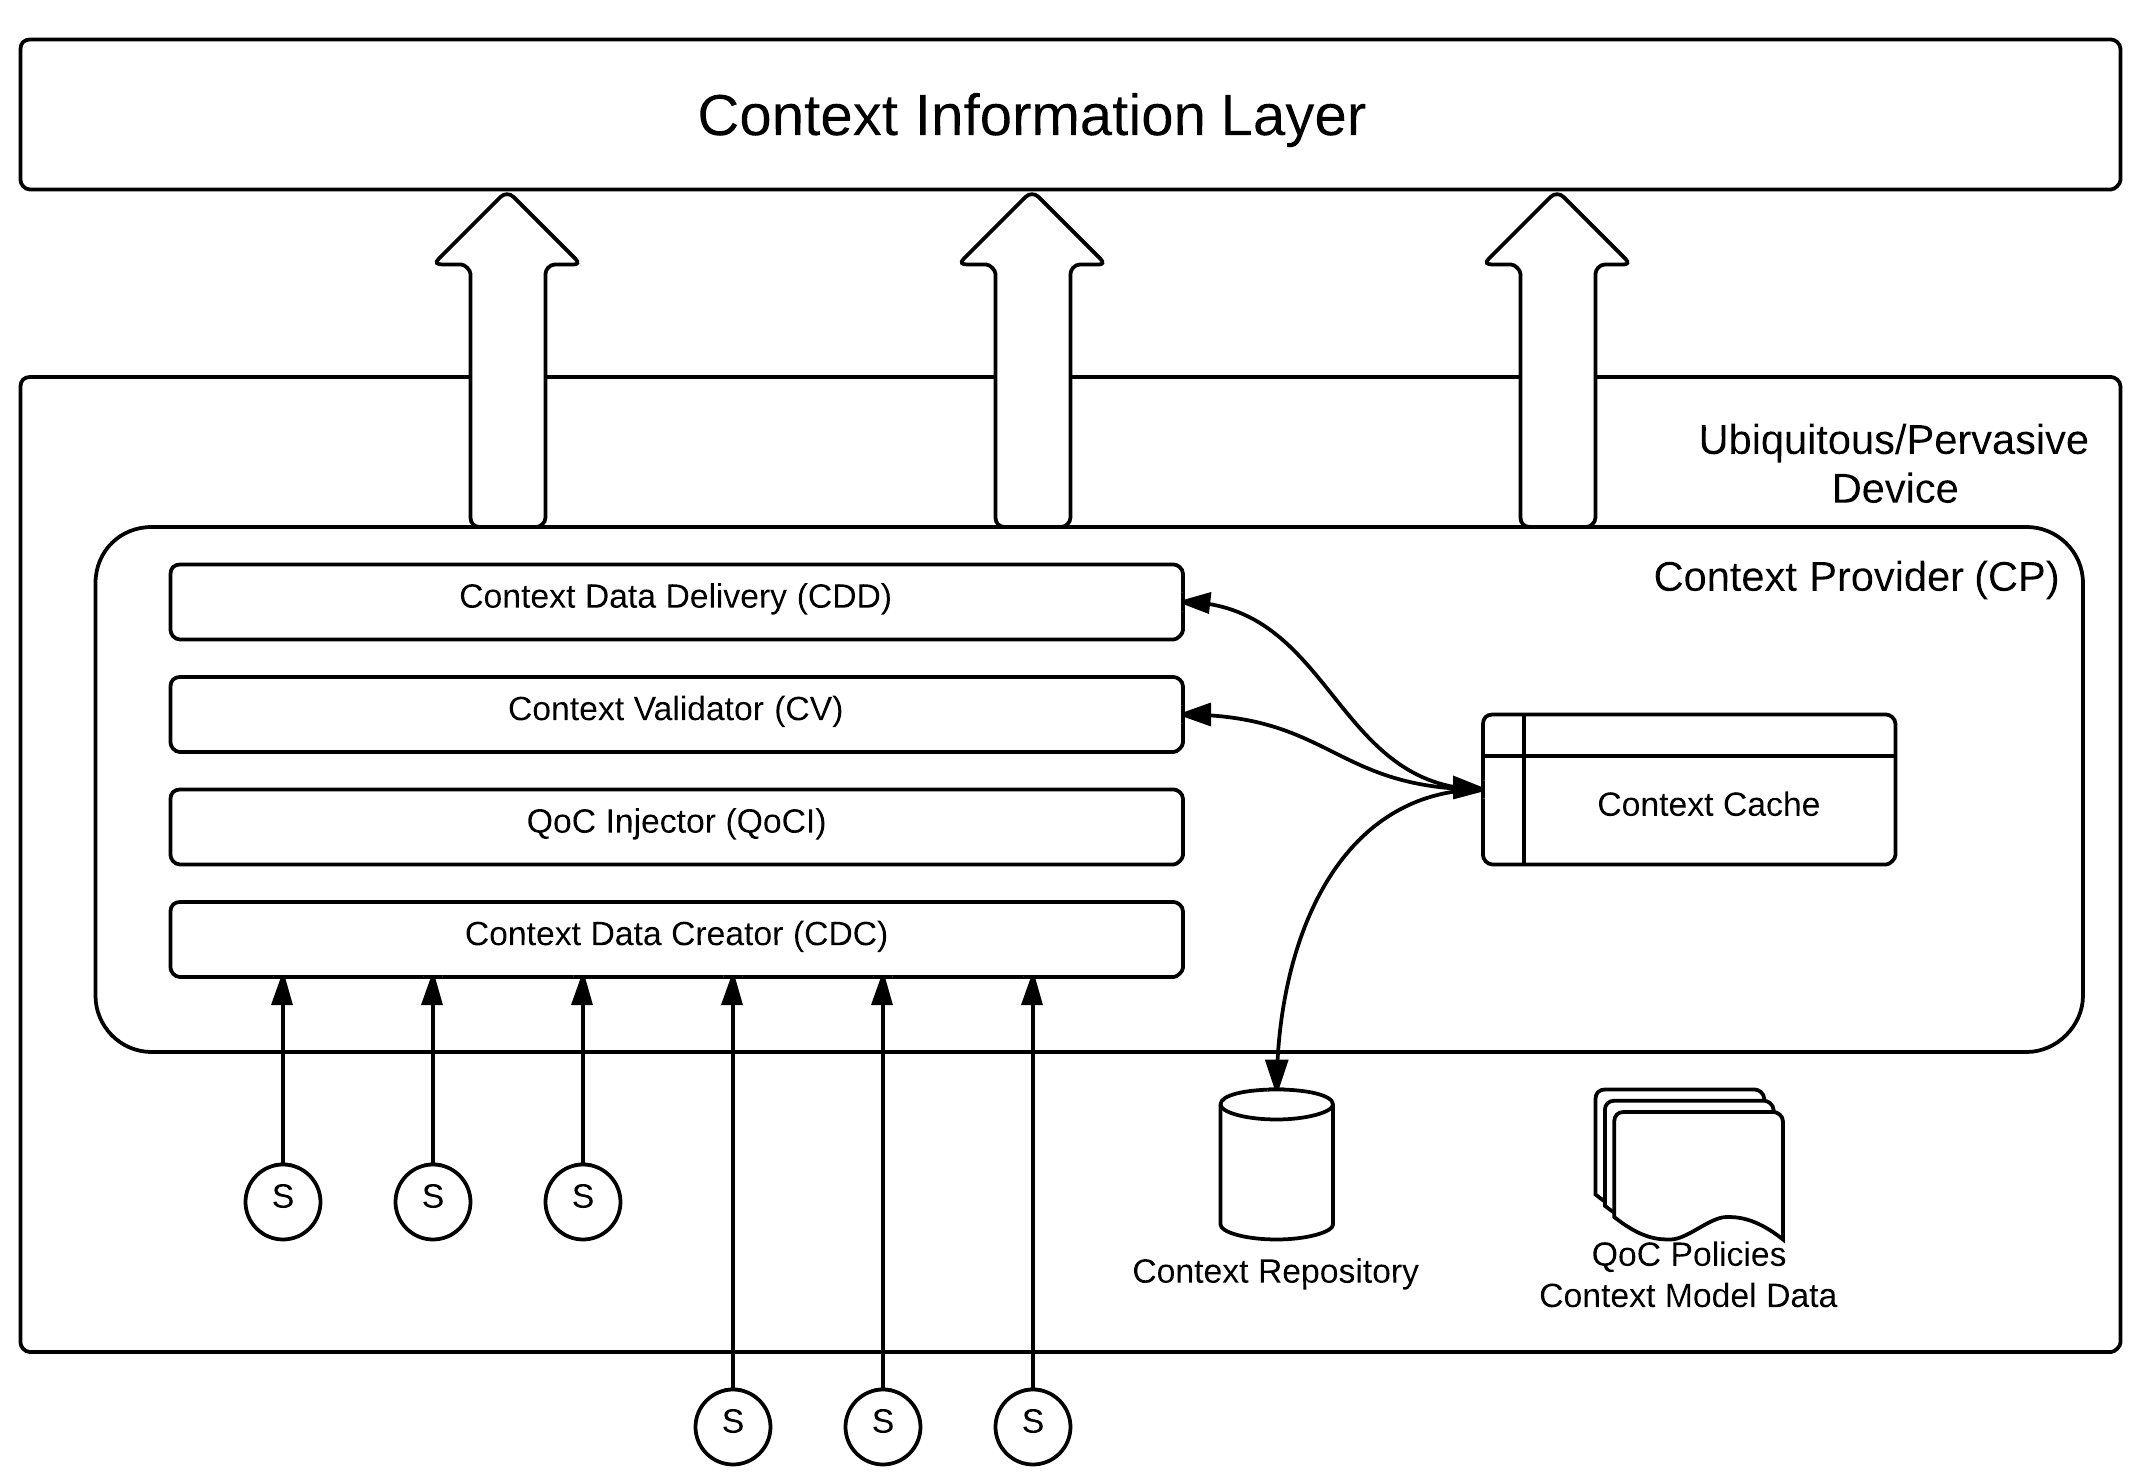
\includegraphics[scale=0.1]{imagens/ClientContextModel}
 \caption{Quality-Aware Context Provider logical architecture}
  \label{qualitymodel}
\end{figure}

\subsubsection{Context Data Creator}

Context Data Creator (CDC) module deals with the specific hardware of a pervasive device.
This module has the function to capture raw information provided by device sensors and 
transform it into interoperable context data to the context middleware. CDC uses context
model definitions to standardize the context information recently received.

On a heterogeneous environment, raw context information is provided by a series of 
different ubiquitous devices, each having its own data pattern. CDC ensures that the 
context provider only send information that can be manipulated in all layers of context
middleware. Consequently, the computational effort performed on the server to convert or
manipulate data, received from various sources, is drastically reduced.

\subsubsection{Quality of Context Injector}

Quality of Context Injector (QoCI) injects QoC parameters in context data. The quality 
parameters are extracted from QoC model. Each quality indicator is related to one or 
more context parameters, in accordance to the definitions set out in QoC policies. This
component discards the newly created context data if it does not have some of the context
information required by the context model. Fragmented context data (and so incorrect) 
must be discarded, since the information contained therein may mischaracterize the 
current real world situation.

It is relevant to mention that QoCI utilizes the concept of completeness to dismiss 
context data. The idea of completeness refers to the availability of information. Thus,
we believe that it is pointless to conduct a computational processing on incomplete data.
Inasmuch as, in fact, no reliable information can be extracted from such data. Therefore,
all policies defined in terms of completeness are previously used by QoCI to eliminate 
incomplete context data.

\subsubsection{Context Validator}

Context Validator (CV) validates context data through the use of QoC policies. For the 
correct use of quality policies, it is necessary that the QoC parameters values are 
already defined. Accordingly, CV is also responsible for evaluating quality parameters. 
The evaluation process can be done in different ways, depending on the policy (static, 
dynamic) in which the QoC parameter is being used.

\begin{itemize}
 \item \textit{Static Policies:}  In this type of policy, QoC parameters values are 
				   pre-defined. CV, then uses the comparison operator 
				   defined in the policy along with the QoC parameter to 
				   evaluate the information in terms of quality of 
				   context.
 \item \textit{Dynamic Policies:} Here, QoC parameters values are dynamic calculated 
				   based on the relation defined on the policy itself. 
				   The comparison operator is also used to evaluate 
				   quality of context on information.
\end{itemize}

 After ensuring quality on the new context data, CV query the context cache collecting 
 all context data recently sent to find and remove redundancies. Some applications may 
 require redundant data to perform further analysis on a given situation. For this 
 reason, the characterization of redundant data is performed through QoC policies. Thus,
 each application can have its own definition of redundant context data.

 The validation process aims to improve the quality of data that are transmitted, 
 ensuring that only meaningful data are sent to applications. However, despite the 
 constant growth in processing power of mobile devices, all validation algorithms and 
 calculations should be designed based on limitations of pervasive device. High 
 complexity algorithms must be performed by the context server layers. Then, when some 
 of the parameters are not pre-defined and demand high computational cost to be 
 evaluated, the server is required to provide the information through the device 
 distribution layer, if necessary.

\subsubsection{Context Cache}
 
 Context Cache (CCa) stores runtime valid context data. Furthermore, the cache 
 communicates with the context data delivery, transferring and requesting valid 
 context data and QoC information, when necessary. CCa also acts as a persistence 
 manager on mobile device, using the device storage space to save context data, thus 
 reducing the number of requests to the context server. Context cache performs 
 operations on Context Repository (CR) to delete invalid data and update values of 
 information.
 
 In ubiquitous mobile environments, it may happen that the context provider is also a 
 context consumer. Applications can adapt more quickly using the information stored in 
 mobile device itself. Furthermore, mobile devices face different computational contexts,
 which can cause connectivity issues, so the cache stores data until the connection is 
 re-established and context data can be sent.
 
 Other important point is related to unnecessary reprocessing that must not happen on a 
 ubiquitous environment given the energetic limitation of mobile devices. Already 
 evaluated QoC parameters, must be maintained and managed by CCa until new values are 
 calculated, thereby preventing rework. QoC parameters that require dynamic and complex 
 calculations to be evaluated, should not be used in context provider policies. The 
 context server is to be responsible to evaluate and use this QoC parameter to ensure 
 the desired quality on context data.
 
 \subsubsection{Context Data Delivery}
 
 CDD distributes device context data to context consumers. Also, when some information 
 cannot be evaluated by the context provider, CDD can receive data from context 
 information layer. This component interacts with CCa in two diferrent situations: 
 i) in case of any connection limitation that may prevent sending context data, CDD 
 stores these data in cache; ii) when CCa requires an information that should be used 
 by CV to perform the validation process, CDD send a request to context information 
 layer. CDD implements all the required coordination and dissemination protocols to 
 carry the published context data to the interested context nodes.
 
 Context Data Delivery was designed to ensure quality of context on data distribution 
 (e.g., data delivery time, reliability,...). Some QoC parameters are defined under 
 temporal aspects (e.g., up-to-dataness, freshness, ...), and delivery delays can alter
 the validity of these data quality parameters. Usually, context data distribution 
 exploits best-effort wireless infrastructures that could introduce delays and 
 droppings \cite{bellavista2013survey} thus, this component was designed to avoid 
 additional inaccuracies in the final context data. 
 
 The presented proposal aims to establish quality of the context in the context provider.
 This can be achieved by exploiting the facilities provided by pervasive devices to 
 perform operations that ensure the delivery of quality data for context-aware 
 applications. Also, QoC policies were defined in order to characterize the scope of 
 relevant information for each application. In a more comprehensive, we intend to 
 improve the quality of transmitted data between context producers and consumers.
 
\section{Experiments and Evaluation}

  In our simulated environment, we used real data from GPS collected from trajectories 
  of four vehicles. The experimental framework, which was based on the work of 
  \cite{martin2009generalized}, is presented on figure \ref{contextcomp}. Vehicles 
  number 1 and 2 were monitored for 3 non-consecutive hours, generating seven different 
  trajectories. Vehicle 3 was monitored for an hour and a half, in a single trajectory.
  Vehicle 4 was monitored during a week totaling 5 hours and 23 minutes of use, 
  generating nine different routes. 
  
   \begin{figure}[!ht]
  \centering
   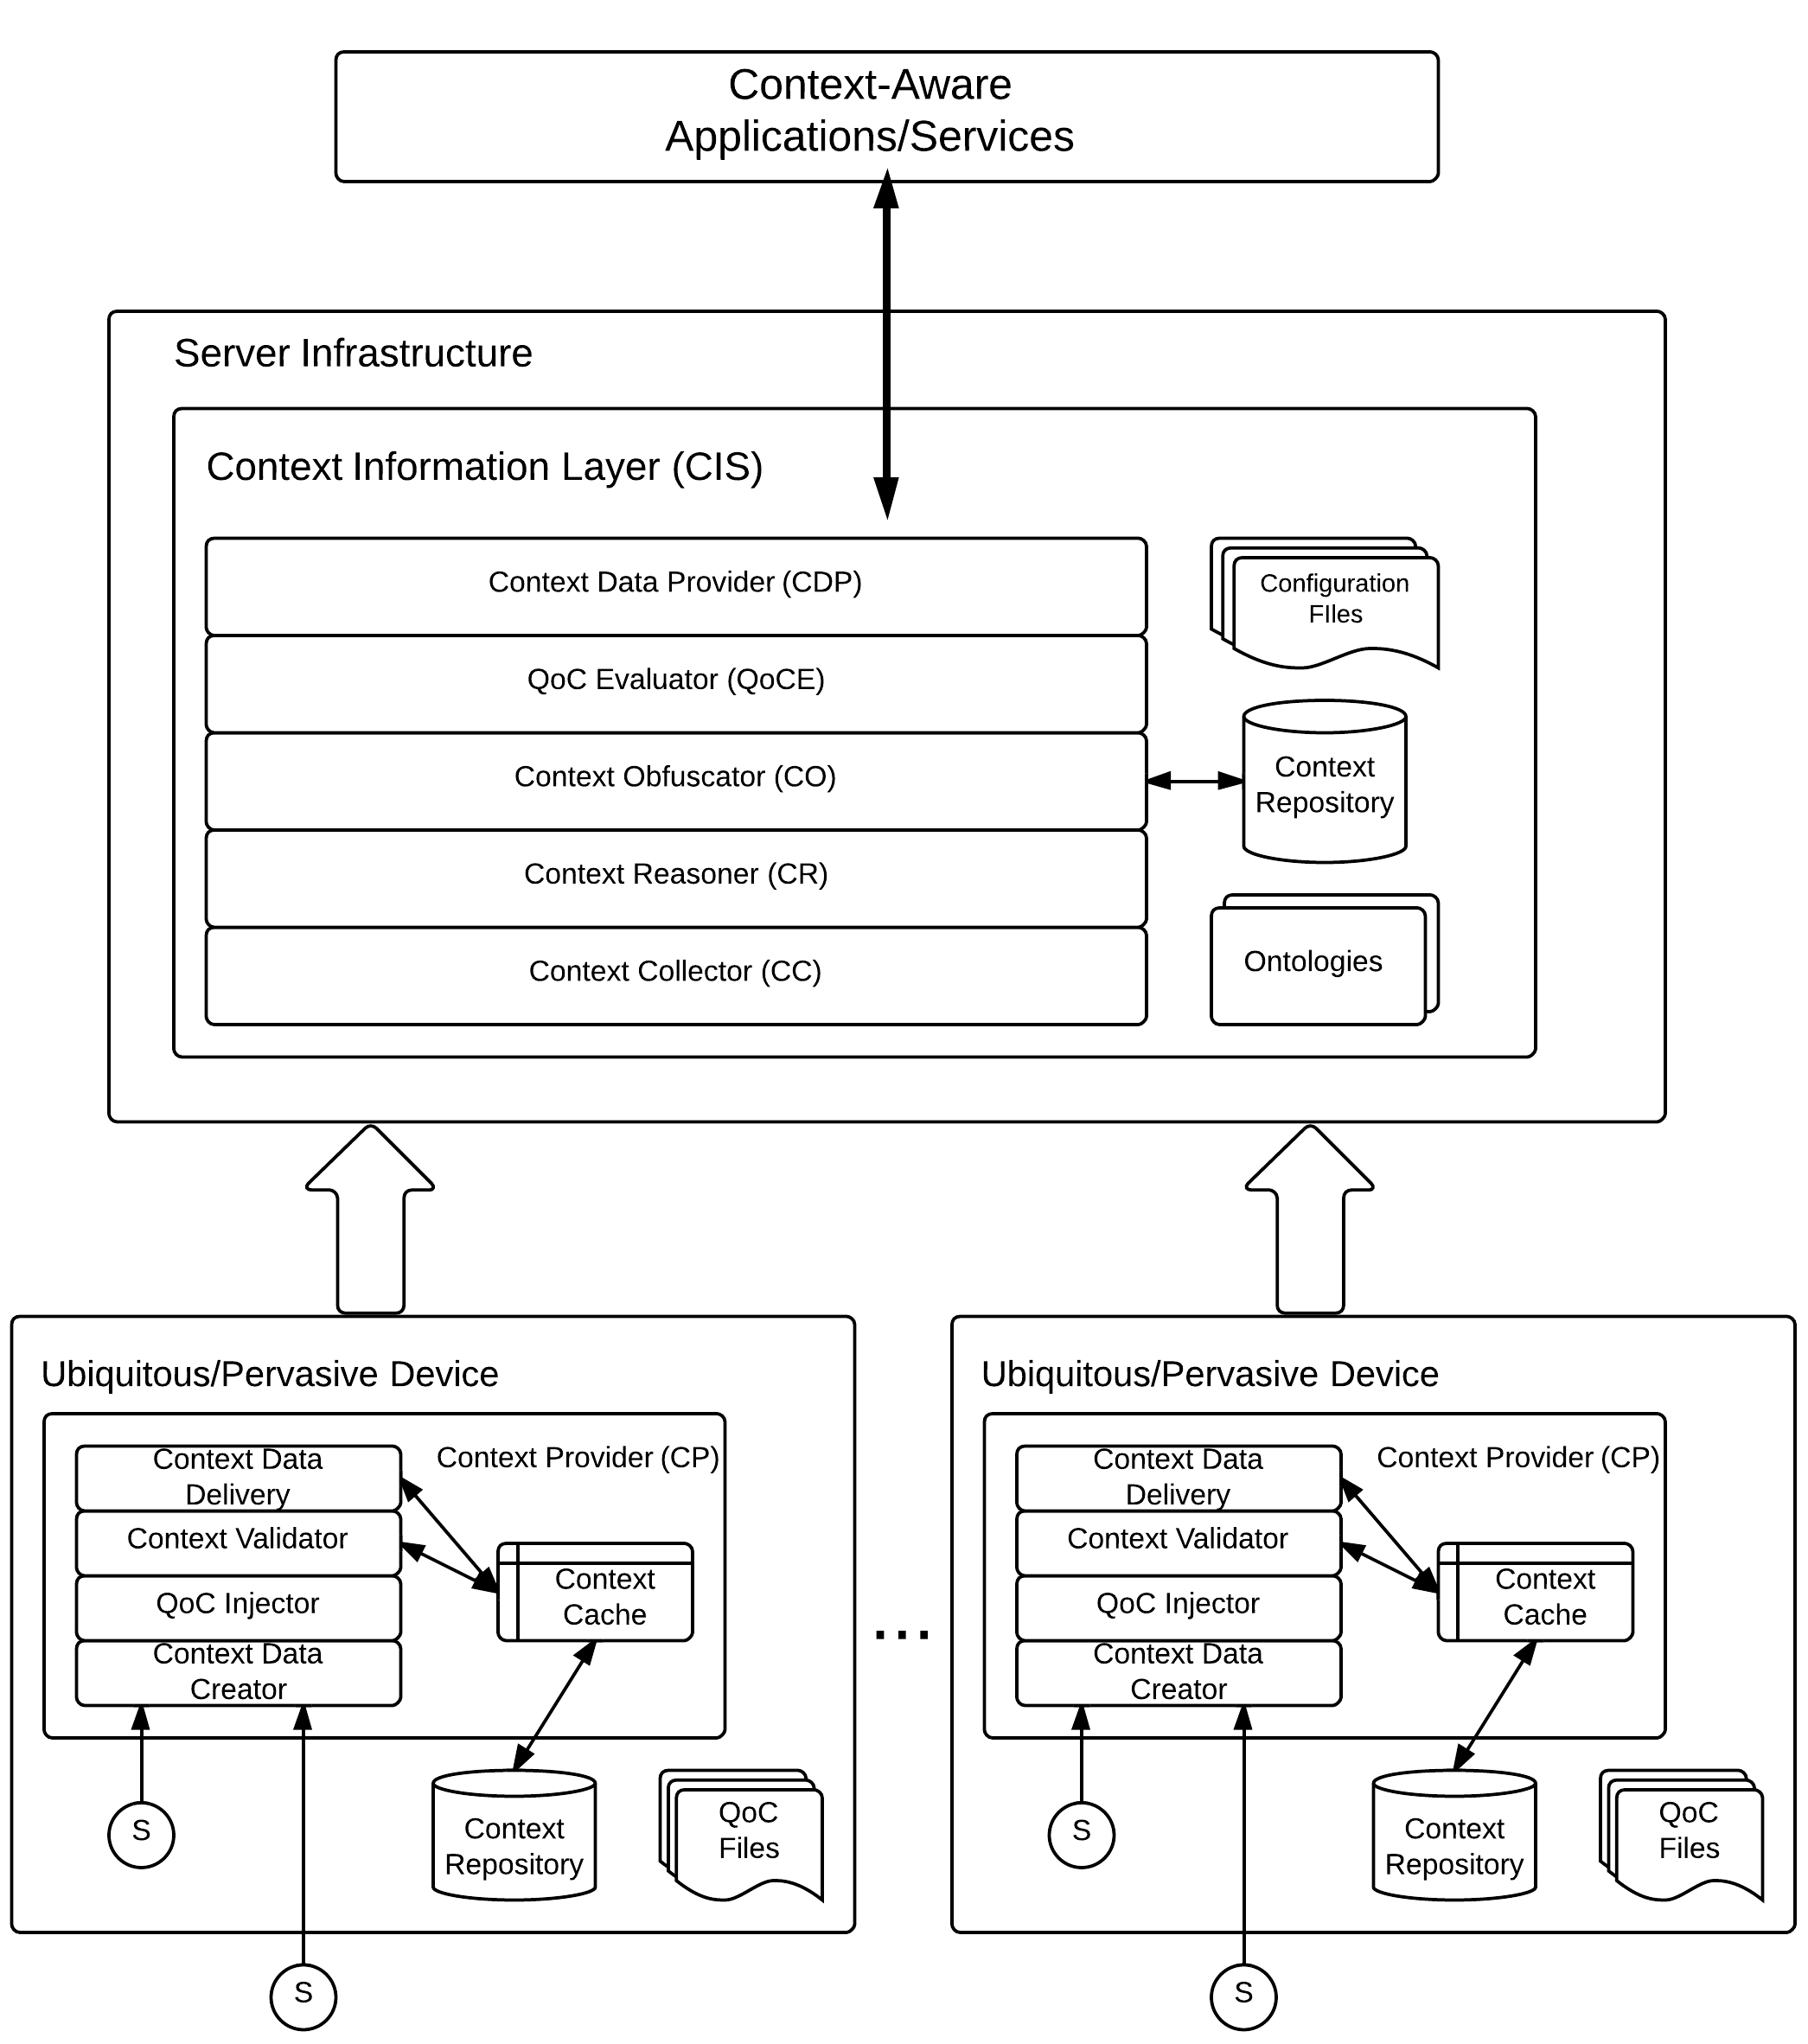
\includegraphics[scale=0.107]{imagens/ContextPlatform}
  \caption{Context-Aware System Components}
  \label{contextcomp}
 \end{figure}
  
  The range of GPS accuracy is 3m to 5km, which is justified by the amount of 
  surrounding buildings, loss of network connection, and limitation of the device itself.
  Thus, this scenario produces a large amount of redundant and conflicting data (e.g. 
  when the vehicle stops or when there is interference in the satellite signal), 
  featuring an actual application for the proposed model. 

  We simulate four pervasive devices sending information uninterruptedly to a context 
  server. The experimental environment is presented on table 1. The context providers 
  were configured to convey context data at an interval of 1-second to context 
  information layer. Besides the geographic information, context providers also 
  provide time and computational context information.
  
  The range of GPS accuracy is 3m to 5km, which is justified by the amount of 
  surrounding buildings, loss of network connection, and limitation of the device itself.
  Thus, this scenario produces a large amount of redundant and conflicting data (e.g. 
  when the vehicle stops or when there is interference in the satellite signal), 
  featuring an actual application for the proposed model. 

  We simulate four pervasive devices sending information uninterruptedly to a context 
  server. The experimental environment is presented on table 1. The context providers 
  were configured to convey context data at an interval of 1-second to context 
  information layer. Besides the geographic information, context providers also 
  provide time and computational context information.

  The adopted policies were: (i) the accuracy of GPS information must be present in 
  context data (ii) the accuracy of GPS data is at most 50 meters, (iii) the distance 
  difference between two consecutive GPS data must be greater than 200 meters and (iv) 
  the time difference between two consecutive GPS data should be greater than 10 seconds.
  Policy file schema is presented in listing 1.
  
   \lstset{basicstyle=\footnotesize\ttfamily\bfseries,
	 breaklines=true
         keywordstyle=\color{black}\bfseries\underbar,
	 identifierstyle=, 
	 commentstyle=\color{white},
	 stringstyle=\ttfamily, 
	 showstringspaces=false}
	 
    \noindent\begin{minipage}{0.475\textwidth}
  \begin{lstlisting}[frame=single, caption=XML representation of a QoC policy file]
   <?xml version= "1.0"?>
   <QoCPolicies>
     <Policy>
       <ParameterName>Latitude</ParameterName>
       <ParameterName>Longitude</ParameterName>
      
       <QualityParameter>
       <Name>Precision</Name>
       <And>
         <IsLessThan>50</IsLessThan>          
	 <IsNull>false</IsNull>         
       </And>  
      </QualityParameter>  
    <Policy>
    
    <Policy>
	<ParameterName>DistanceDifference</ParameterName>
	<IsGreaterThan>200</IsLessThan>          
	<IsNull>false</IsNull>         
    <Policy>
    
    <Policy>
       <ParameterName>TimeDifference</ParameterName>
       <IsGreaterThan>10</IsGreaterThan>
    <Policy>
 </QoCPolicies> 
    \end{lstlisting}
  \end{minipage}
  
 \begin{center}
 \begin{table*}[!t]
  \scriptsize
	\begin{tabular}{|p{1.6cm}|p{1.6cm}|p{1.6cm}|p{1.6cm}|p{1.6cm}|p{1.6cm}|p{1.6cm}|p{1.6cm}|}
	\hline
	\textbf{} & 
	\textbf{Operational System} & 
	\textbf{Processor} &
	\textbf{Memory} &
	\textbf{Storage} & 
	\textbf{Database} & 
	\textbf{Programming Language} &
	\textbf{Environment}\\ \hline
	    Context Providers    & Android 4.1 & Quad-core 1.4 GHz & 512MB  & 16GB & GvSig 0.3 & Java 1.7 & Android Emulator \\ \hline 
	    Context Server	    & Ubuntu 12.04 64-bit & Intel i5 2.5GHz & 4GB & 1TB & PostGIS 2.0 & Java 1.7 & Dell Vostro 3460 \\ \hline
	\end{tabular}
   \caption{Experimental environment}
   \label{tab:nonfloat}
  \end{table*}
 \end{center} 
  
  Figure \ref{objectsent} shows the number of context data filtered in 6 hours 
  simulation. Both, QoC parameter policies and application policies reduced the 
  number of context data transmitted. Our intent here was to show the effectiveness 
  of the policies separately, as a policy does not interfere with each other.
  
 \begin{figure}[!h]
  \centering
  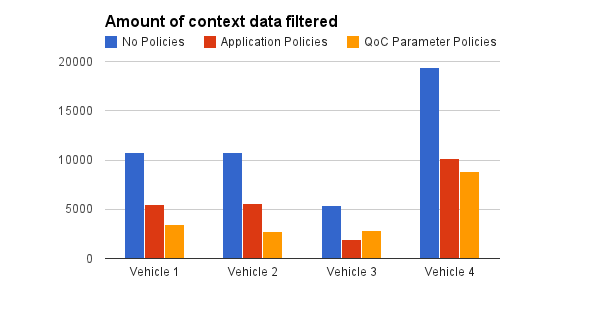
\includegraphics[scale=0.35]{imagens/amountdata}
  \caption{Amount of filtered context data}
  \label{objectsent}
 \end{figure}
  
  Figure \ref{non-filtered} shows data without any context filtering procedure. 
  Unfiltered data represent trajectories that differ from the trajectory actually made 
  ​​by user. Figure \ref{filtered} shows the same route shown in figure \ref{non-filtered}, 
  however, with filtered data. The amount of data representing the trajectory was decreased
  by approximately 40\%
  
  For a better visibility, we chose not to represent the trajectories as a whole because,
  on average, each trajectory is represented by 4000 points. For this reason, we chose to
  evaluate an excerpt from the trajectory which had stop and signal loss situation, since
  these stretches of the trajectory concentrate a large number of redundant and 
  conflicting data. It is noticed that with unfiltered data is hard to see the route 
  itself, the data set does not seem to represent a trajectory.
  
\begin{figure}[!h]
 \centering
  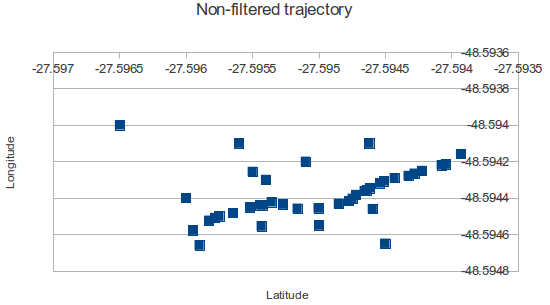
\includegraphics[scale=0.35]{imagens/NonfilteredTrajectory}
 \caption{Non-Filtered Trajectory}
 \label{non-filtered}
 \end{figure}
 
  \begin{figure}[!h]
 \centering
  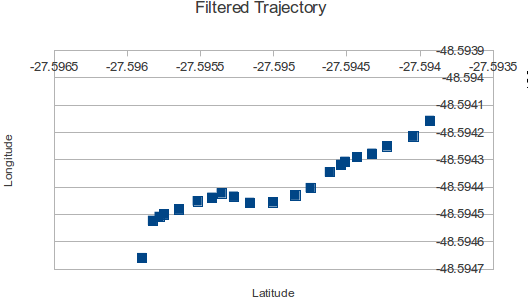
\includegraphics[scale=0.35]{imagens/FilteredTrajectory}
  \caption{Filtered Trajectory}
  \label{filtered}
 \end{figure}
 
 This combination of findings provides some support for the conceptual premise that 
 quality of context only can be fully assure if the requirements of each application 
 are designed in context model and that mobile devices can be used to ensure a better 
 quality of context. The overall behavior of our simulated experiments show that the 
 approach reduces the number of data transmitted and also improved the trajectory 
 representation. We have also observed that policies defined in the need of that 
 specific application tends to better attend context-aware services requirements.
 
\section{Conclusion}

 The research work presented in this paper proposes an enhanced filtering approach for 
 ubiquitous environments. The model was grounded in the fact that the pervasive device 
 is an important part for the process of quality and therefore it is, also, responsible 
 for guaranteeing it. Filters on mobile devices are responsible for all context objects,
 eliminating redundancy and conflicts before the data is sent to context server. As a 
 result of the proposal, experiments indicated that the amount of data sent significantly
 reduced and the trajectories were better represented with filtered data.

 As a future work, we aim to exploit semantic aspects that involve context data in order 
 to define more robust policies. In addition, a context model with greater granularity 
 is desirable, improving the context information export procedure from mobile device. 
 Experimental tests will also be conducted with a larger number of applications 
 in a more heterogeneous environment, with the objective of identifying possible 
 improvements and limitations on the proposed approach. Finally, we intend to conduct a 
 performance study verifying the time overhead added by the Quality-Aware Context 
 Producer approach and a device’s battery analysis during the context data transmission.

\bibliographystyle{IEEEtran}
\bibliography{bare_conf(copy)}

\end{document}


